\documentclass[noheader]{coursclass}

\usepackage{tikz-repère}
\usepackage{tkz-tab}
\usepackage{tabularx}

\begin{document}

\begin{greybox}[frametitle={Fonctions carrée et cube}]
	\begin{center}
		\begin{tabularx}{0.9\linewidth}{>{\raggedright\arraybackslash}X|>{\raggedright\arraybackslash}X}
			La fonction \textbf{carrée} est la fonction $$f(x) = x^2$$                   & La fonction \textbf{cube} est la fonction $$g(x) = x^3$$          \\
			                                                                             &                                                                   \\
			Pour tout nombre réel $x$, on a \hspace{8em} $$f(x) = f(-x)$$                & Pour tout nombre réel $x$, on a \hspace{5em} $$g(-x) = -g(x)$$    \\
			                                                                             &                                                                   \\
			\textit{L'axe des ordonnées} est un axe de symétrie du graphe.               & \textit{Le centre du repère} est un centre de symétrie du graphe. \\
			                                                                             &                                                                   \\
			\begin{center}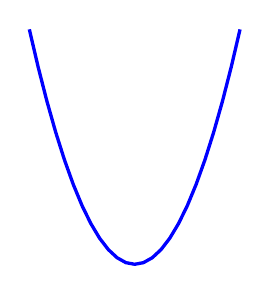
\begin{tikzpicture}[scale=0.6]
					\tikzRepere{-2.5}{2.5}{-0.5}{4.5}
					\draw[very thick,blue,domain=-2.23:2.23] plot({\x},{\x*\x});
				\end{tikzpicture}\end{center}
			La courbe est une \correctionDots{\textbf{parabole}}. \medskip

			Le point de coordonnées $(0; 0)$ est le \correctionDots{\textbf{sommet}} de cette parabole. & \begin{center}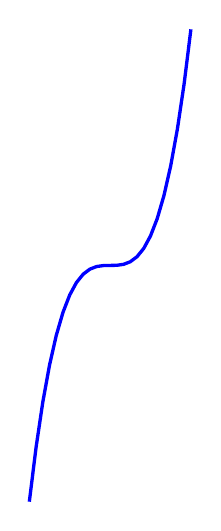
\begin{tikzpicture}[scale=0.6]
					\tikzRepere{-2.5}{2.5}{-4.5}{4.5}
					\draw[very thick,blue,domain=-1.71:1.71] plot({\x},{\x*\x*\x});
				\end{tikzpicture}\end{center}               \\
			Tableau de variations :

			\begin{center}\begin{tikzpicture}[scale=0.7]
					\tkzTabInit{$x$ / 1 , $x^2$ / 2}{$-∞$, $0$, $+∞$}
				\end{tikzpicture}\end{center}                          & Tableau de variations :

			\begin{center}\begin{tikzpicture}[scale=0.7]
					\tkzTabInit{$x$ / 1 , $x^3$ / 2}{$-∞$, $+∞$}
				\end{tikzpicture}\end{center}
			\\
		\end{tabularx}
	\end{center}
\end{greybox}

\end{document}